\chapter{背景}
\label{chap:relevantstudy}

本章では麻雀のゲーム理論的な位置づけと、AIを作る上で課題となる点を述べる。また、麻雀の一般論や関連研究についても同様に述べる。

\section{麻雀のゲーム理論的分類}
昨今では、Googleが囲碁の世界で世界チャンピオンを破ったことは記憶に新しく\cite{go}、あらゆるゲームAIが様々な分野で活躍している。二人零和有限確定完全情報ゲームに分類されるチェス、将棋、オセロ、囲碁などは既にトップレベルの実力を達成している。これらのゲームはまず、二人零和ゲームであるために、自分の得点と相手の得点の関係性が明確である。自分の得点はすなわち相手の失点と等価であり、また、自分の失点は相手の失点と等価である。そのため、自分を有利な立場にするような戦略のモデルが作りやすく、これらの研究はいい結果を残している。また、有限であることも重要である。ゲームが有限な手数で終わるということがわかっている場合、モンテカルロ法によるシミュレーションなどで最終スコアから手の良さを逆算することが可能であるからである。これが無限になるケースだと、探索範囲が無限に広がるどころか、ゲーム終了時のスコアを取れない場合があるので難しい。さらに、確定完全情報ゲームであることは、ゲームの複雑性を少なくすることにおいて大切である。手の選択によって得られる結果が確定でないゲームでは、特定の手によって起こる結果をモデル化すること自体研究対象となる。また、不完全情報ゲームでは、相手プレイヤーや場のモデルも構成しないといけないため、同様に複雑性を増す。
\\本研究の対象となる麻雀は、分類するとしたならば、四人零和有限不確定不完全情報ゲームである。以上に述べたような二人零和有限確定完全情報ゲームと異なり、課題が多いために麻雀のAIは未だにトッププレイヤーレベルの実力に達しているものは存在しない。まず際立つ問題がプレイヤーが4人という多人数であることである。2人プレイヤーでは自分の得点と相手の失点は等価であったが、4人プレイヤーの場合自分と特定の相手プレイヤーの得点の関係は同様ではない。すなわち、プレイヤーごとに達成すべき目的が異なる場合が存在するため、単純なモデルを作ることが難しい。この多人数性の問題を解決するには、プレイヤーを1人とした1人麻雀の利用が考えられる。これは、麻雀プレイヤーが自分の実力を高めるために練習として使う用途があったが、水上ら\cite{bakuuti}などが麻雀の研究をする際に使用している。本研究でも、評価としてこの1人麻雀を利用する。次に、不確定性が存在する面も、麻雀のAIを作る際に難しい問題となっている。選択した手によって得られる結果が確定でない以上、これらは確率的にしか求めることが出来ない。この問題に対してのアプローチとしては、途中局面のヒューリスティクスを用いて手の優劣を決定する手法の他に、モンテカルロ法によるシミュレーションを用いた方法などが挙げられる。本研究では前者を対象とするが、これらの関連研究については次節以降に解説する。

% プレイ人数に着目した研究としてはポーカーを用いたもの \cite{poker},\cite{hurui} がある。これらの手法では 2 プレイヤでのゲームを強くしてから多人数に適応する方法がとられている。ポーカーは2 プレイヤであればナッシュ均衡戦略を用いることで世界チャンピオンに勝っているが、ポーカーは 2人から 10 人程度で参加可能なゲームであり人数が増える
% と状態数が指数関数的に増大するためナッシュ均衡戦略の計算は難しい。そこで 2 人で行われたナッシュ均衡戦略を3 人限定で拡張する方法、プレイヤの行動を削減、抽象化することでより少ない人数の少ないゲームを想定する方法がとられた。

\section{麻雀の一般論}
この節では麻雀の一般論について述べる。前節で述べたように、麻雀は多人数性と不完全情報の観点から、複雑さを極めるルールとなっている。ただし、戦略について大きく分けると、自分の得点を加算する攻めの技術と、失点を防ぐための守りの技術に分類することができる。これについてこの節では解説する。また、本研究では攻めについて取り扱うため、攻めの戦略において重要である指標についても説明する。
\subsection{押しと降り}
一般に、麻雀において攻める技術の押し、守る技術のことを降りという。麻雀で得点を加算することは、原則自分の手を和了ることによってのみ実現される。したがって、押しの技術に関してはまず自分の手を和了まで持っていけるかということが重要となる。和了の形式としてはツモ和了とロン和了が存在し、ツモ和了では他の相手プレイヤー全てから得点を奪い、ロン和了では上がり牌を河に捨てたプレイヤーから得点を奪う。次に、和了の形、すなわち役によって加算される際の得点が異なるため、できるだけ高い打点の構成で上がることが求められる。
\\一方、麻雀で失点となる局面は、原則相手プレイヤーが和了した時である。失点の方式は2つあり、放銃失点と被ツモ失点によるものである。前述した相手プレイヤーがロン和了となるような牌を自分が河に捨ててしまった場合は放銃失点となり、相手プレイヤーがツモ和了した場合は被ツモ失点として得点を支払う。ただし、被ツモ失点の場合は他プレイヤーとともに失点を痛み分けすることになるので、放銃失点よりは失う得点が少ない。したがって、被ツモ失点は免れることは難しいが、放銃失点は自分の捨てる牌に注意することで免れることが可能となるため、降りの戦略としては主に相手プレイヤーをロン和了させないように打つことが基本となる。

\subsection{シャンテン数}
和了形は役によって多少の違いはあるが、一般に雀頭1つとメンツ4つで構成される。この形を、与えられた13牌の配牌から始め、山から1枚ツモり自分の手牌から1枚切る動作を繰り返すことで完成させることが和了となる。ここで、まだ和了形に至っていない牌姿において、和了までどれだけの距離があるかを示すための指標としてシャンテン数が存在する。シャンテン数とは、実際には和了形ではなくその一つ手前の状況である聴牌を基準としたものであるが、基準としては和了までの距離として使って構わない。シャンテン数の具体的な定義は、現在の牌姿から最短何回のツモで聴牌にたどり着くことができるかをである。具体例を図\ref{2syanten}に示す。この場合は、最短であと3つの必要な牌をツモることで和了することができ、あと2つの必要な牌をツモることで聴牌であるため、この牌姿は2シャンテンである。

\begin{figure}[h]
 \centering
 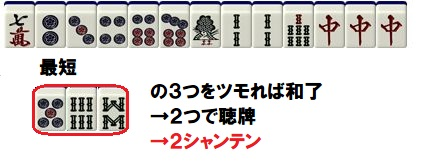
\includegraphics[keepaspectratio, scale=1,bb=0 0 320 239]
      {img/2syanten.jpg}
 \caption{シャンテン数}
 \label{2syanten}
\end{figure}

\section{関連研究}
和了率を高めるための研究としては大きく分けて、強者の牌譜を学習してモデルを作る方法、モンテカルロ法によるシミュレーションを用いた方法、途中局面のヒューリスティクスを用いた方法があげられる。強者の牌譜を学習してモデルを作る方法では水木ら\cite{miki}や北川ら\cite{kitakawa}、水上ら\cite{bakuuti}の研究が報告されているが、いずれも面前においての和了率は平均プレイヤの実力に至っていない。これらは、4人麻雀の牌譜を使っていることで、4人麻雀独特の打ち方を排除できない問題や、上級者が認知できない最適解を求められない問題があった。また、モンテカルロ法によるシミュレーションを用いた方法では、麻雀は分岐が多すぎるため探索範囲が広く、そのまま適用しても精度が出ない。したがってこの分野の研究としては、探索範囲を限定することができるUCB\cite{UCB}やUCT\cite{UCT}と言った手法が利用されている。UCBを利用した打牌アルゴリズムとしては中張らの研究が\cite{LinUCB_mahjong}あげられる。また、UCTを利用した打牌アルゴリズムでは、三木らの研究が\cite{miki}挙げられる。これらはそれぞれの手法によって探索範囲を限定したシミュレーションを行っているが、麻雀の分岐局面が多すぎる問題に対してまだ課題が多く、平均プレイヤーを超える和了率は出せていない。最後に途中局面のヒューリスティクスを用いた方法だが、面前の和了率を上げるためにはいい成績が出ている。この分野での研究としては、佐藤らの有効牌を数え上げることによって打牌するアルゴリズム\cite{zentsu}などがあげられる。相手プレイヤーに関する鳴きや打点などを考慮した観点からは劣る部分も多いが、面前の和了率については良い結果を残している。これらの研究は、本研究の手法と近いため、詳しく次章でまた解説する。



% \section{関連研究}
% \subsection{UCB1}
% 以上で述べたモンテカルロ法の問題点は、各ノードに対して行うシミュレーションがそれぞれ膨大なため、プレイアウトまでの回数が多く精度が落ちてしまうことである。
% この問題を解決するために、提案されている手法の中に、Upper Confidence Bound (UCB) \cite{UCB}を用いたものがある。
% UCB ではある局面から考えられる全ての手に対して, よい結果 を返しそうな手を重視しつつ、何度もプレイアウトと呼ば れるランダムシミュレーションを行うことで 最善の手を決定する手法である。有望な手に対して多くのプレイアウトを実行することで、先に述べた通常のモンテカルロ木探索よりも精度を上げることができる。以下、このアルゴリズムを詳しく説明する。

% 通常のモンテカルロ木探索では、ノードごとに期待される手の良さを途中で判定していないため、全てのノードに対して同じ回数のプレイアウトを行うことになる。したがって、良い手が期待できないノードに対しても多くのプレイアウトを割り当てることになり、無駄なシミュレーションを行ってしまう事が考えられる。また、ノードによっては手の良さを決定する分岐がプレイアウトに対して大量にある場合、他のノードと同じ回数のプレイアウトでは十分な評価が出来ない可能性もある。このような問題に対して、UCBでは、UCB1値を用いることによって各ノードの有望さをその都度確認し、全体のプレイアウトの回数や特定のノードで行われたプレイアウトの回数を考慮して、プレイアウトをどのノードに数多く割り当てるかということを判別することを考える。
% UCB1値は、${x_{j}}$は子ノード$j$の平均報酬, $α$は定数,$n$は親ノードの探索回数, ${n_{j}}$は子ノード$j$とした時、

% \begin{equation}
% \label{UCB1value}
% \Large UCB1 = \overline {x_{j}}+\alpha \sqrt {\displaystyle \frac {2\log{n}} {n_{j}}}
% \end{equation}
% で表される。
% 式 \ref{UCB1value}の右辺の第 1 項は平均報酬を, 第 2 項は信頼度を示している。従来のモンテカルロ木探索では第1項の平均報酬をそのまま全てのプレイアウトが終了するまで行った値として利用していたが、UCB1ではここで第2項の信頼度を用いることで全てのプレイアウトが終了するよりも前に信頼できる範囲を推定する。そうすることで、多くのプレイアウトを最後まで割り当てなくとも、一定の信頼度で少ないプレイアウトでそのノードが有望かどうかを判別することが可能になる。
% 信頼度はそのノードのプレイアウト回数が少ないと大きく, 多いと小さくなる。UCB1 値を用いることでUCB1 ではよ り有望そうな手に対して多くのシミュレーションを行う事 ができる。

% \begin{figure}[h]
%  \centering
%  \includegraphics[keepaspectratio, scale=0.75,bb=0 0 304 387]
%       {img/UCB.png}
%  \caption{UCBを用いたモンテカルロ木探索}
%  \label{monte2}
% \end{figure}

% \subsection{Lin UCB}
% UCB1 は各局面ごとにこの手順を実行するが, 各局面を完全に異なる局面として扱うため, 他の局面の探 索において得られた情報を共有することができないという 欠点を持つ. この欠点を補うアルゴリズムとして期待され ているのが LinUCB である.

% UCB は局面ごとにこの探索を実行するが, 各局面を完全 に別の局面として扱うため他の局面の探索において得た情 報を利用することができない。この問題を解決するためにLinear UCB (LinUCB) \cite{LinUCB} という手法が提案されている。これは、局面を特徴で表す ことで、対象とする局面が異なっても, それまで対象とした局面の情報を利用できるといったものである。

% LinUCB [5] は, UCB を局面を特徴で表すことができる ように拡張したものであり, 牌譜の局面からの教師あり学 習や異なる探索の結果の共有ができる手法である。
% LinUCB はプレイアウトを行う子ノードを選択する評価値の計算に, 重みベクトル, 特徴ベクトル, 特徴の頻度を表す相関行列を 用いる. 計算により求めた評価値が最大となる子ノードに 対してプレイアウトを行い, 共通で保持する重みベクトル を更新する. 重みベクトルは, 選択したノードの特徴ベクト ルの各項にプレイアウト結果の報酬を乗じた値を, 重みベ クトルの対応する項に足し込んで更新する. この更新によ り, 高い報酬を得た特徴は大きな重みを, 低い報酬の特徴は 小さな重みを持つようになるため, 当該ノードだけでなく, 同様の特徴を持つ他のノードの評価値も更新される. これ により異なる局面で得られた情報を共有し, 利用すること ができる. また LinUCB は探索を行った結果を重みベクト ルとして記録しておくことで, 事前学習の結果を用いる探 索として利用することも可能である.
% LinUCB のアルゴリズムを Algorithm 1 に示す. ただし xt,at はプレイアウト回数が t 回目の時の選択肢 a の特徴ベ クトル, A は特徴の共起を含めた頻度を表す相関行列, b は
% 各ノードごとの報酬の総和を表すベクトル, θt は重みベク トル, pt,a は選択肢 a の評価値, α はバランスパラメータ, rt は報酬を表している. rt はプレイアウトにより与えるか, 学習データにより与えるものとする. LinUCB は 4 行目で 前回のプレイアウト結果を反映して重みベクトル θt を更 新する. 7 行目で重みベクトル, 特徴ベクトル, 相関行列を 用いて各ノードの評価値を計算し, 9 行目で評価値が最大 となるノードを選択する. 10 行目でプレイアウトを行い報 酬を受け取り, 11 行目, 12 行目で A と b の更新を行う.
% LinUCB は Algorithm 1 の 7 行目に示したように, 式 (2) により各ノードの評価値を求める. 式 (2) の第 1 項は各ノー ドの平均報酬を計算しており, 第 2 項で信頼度を計算して いる.
% \begin{equation}
% \label{LinUCB}
% \Large pt,a = θTt xt,a + α
% \end{equation}
% また, UCB で用いている評価値も, 平均報酬と信頼度の和 で計算される. つまり LinUCB と UCB は本質的に等しい 計算をしていることが分かる. また, LinUCB の第 2 項は データ数の増加により十分速く小さくなることが保証され ている [5]. 以上より, LinUCB は UCB と近い運用を行う ことができると考えられる.

% これらは麻雀について適用した例が報告されている\cite{LinUCB_mahjong}が、いずれの方法も平均プレイヤーに満たない成績となった。

% \section{本論文が着目する課題}
% 1人麻雀においてある局面からゲーム木を展開しようとした場合、次にどの種類牌をツモるかはわからないため、ランダムに決定しノードを展開していくことになる。これを繰り返し行うと探索空間が大きくなりすぎるため、手の選択が難しくなる。これを対処するために、あらゆる手法が提案されている。このような場合に木を展開せずに有望な手を選択する手法として、Upper Confidence Bound (UCB) \cite{UCB}がある。UCB ではある局面から考えられる全ての手に対して, よい結果 を返しそうな手を重視しつつ、何度もプレイアウトと呼ば れるランダムシミュレーションを行うことで 最善の手を決定する手法である。
% UCB は局面ごとにこの探索を実行するが, 各局面を完全 に別の局面として扱うため他の局面の探索において得た情 報を利用することができない。この問題を解決するためにLinear UCB (LinUCB) \cite{LinUCB} という手法が提案されている。これは、局面を特徴で表す ことで、対象とする局面が異なっても, それまで対象とした局面の情報を利用できるといったものである。以上のような対策が考えられてはいるが、1人麻雀について適用した結果平均プレイヤーの実力までに至っていない。囲碁においては一定の成果を上げたものの、麻雀ではうまく適用できない問題に対しては、麻雀の場合はより探索の空間が大きく、UCB1値やLinUCBを指標とするノードの展開の方法ではうまく適用できていない可能性がある。したがって本研究では、ノードの展開を行う際に指標とするものを麻雀というゲームの性質上の状況のパラメーターを用意し、それを使うこととする。

% しかし、UCB1 と LinUCB の評価値計算において信頼度の 計算式が異なることや、特徴量の設計に問題があるなどの理由でいい結果は出ていなかった。 
